\documentclass[a4paper]{article}

\usepackage{parskip}
\usepackage{amsmath}
\usepackage{amssymb}
\usepackage{amsthm}
\usepackage{tikz}

\theoremstyle{definition}
\newtheorem{definition}{Definition}[section]
\newtheorem{lemma}{Lemma}[section]
\newtheorem{theorem}{Theorem}[section]

\usetikzlibrary{perspective}
\usetikzlibrary{3d}

\tikzset{region style/.style={draw,fill=blue!10,even odd rule}}
\tikzset{rnode/.style={,every node/.style={inner sep=1pt, circle, fill=black, opacity=1}}}

\title{Notes on Boundary Representation}
\author{Birk Tjelmeland}

\begin{document}
\maketitle

\section{Definitions}

\subsection{Spaces}

We define a space $\mathcal{S}$ of $n$ dimensions as a pure manifold of $n$ dimensions 

% TODO: potential alternative definition
A space $\mathcal{S}$ is a set of points of $n$ dimensions with the following requierments:
\begin{itemize}
    \item For any point $P_A \in \mathcal{S}$ and an arbitrary small distance $d$ there exists 
\end{itemize}

TODO: replace all of this stuff with a good external definition of a space with the properties we require.
Metric space? Manifold? 

A space $\mathcal{S}$ in $n > 0$ dimensions can be \emph{segmented} into two parts by a subspace $\mathcal{B} < \mathcal{S}$ of $n-1$ dimensions.
A subspace $\mathcal{B} < \mathcal{S}$ has a mapping $\sigma_\mathcal{B} : \mathcal{B} \rightarrow \mathcal{S}$ that maps any point $P \in \mathcal{B}$ to a point $\sigma_\mathcal{B}(P) \in \mathcal{S}$.
For any point $P \in \mathcal{S}$ and a subspace $\mathcal{B} < \mathcal{S}$ we say that $P$ can either be on the \emph{inside} of $\mathcal{B}$, on the \emph{outside} of $\mathcal{B}$.
A space $\mathcal{S}$ in zero dimensions has a single subspace $\mathcal{B} = \mathcal{S}$.
Two distinct spaces $\mathcal{S}_A$ and $\mathcal{S}_B$ are either \emph{disjoint} or they \emph{intersect}.
We say that two distinct spaces $\mathcal{S}_A$ and $\mathcal{S}_B$ intersect if there exists at least one point $P$ in $\mathcal{S}_A$ that also exists in $\mathcal{S}_B$.
For two spaces $\mathcal{S}_A$ and $\mathcal{S}_B$ that intersect we define their \emph{intersection} $\mathcal{S}_A \cap \mathcal{S}_B$ as the subspace $\mathcal{B}$ such that for each point $P$ in $\mathcal{B}$ a coresponding point exists in both $\mathcal{S}_A$ and $\mathcal{S}_B$.
If the two spaces do not intersect we define their intersection as $\mathcal{S}_A \cap \mathcal{S}_B = \varnothing$.

A path $P$ in a space $\mathcal{S}$ is a set of points an TODO: fix this definition.
The \emph{endpoints} of a path $P$ TODO: depends on definition of path.
A \emph{crossing} $C_\mathcal{B}(P)$ of a path $P$ through a subspace $\mathcal{B} < \mathcal{S}$ is a subpath of $P$ that starts with a point on the outside of $\mathcal{B}$ and ends with a point on the inside of $\mathcal{B}$ and where all other points of $C_\mathcal{B}(P)$ is in $\mathcal{B}$.
The \emph{crossing endpoints} of a crossing $C_\mathcal{B}(P)$ are the endpoints of the subpath of $C_\mathcal{B}(P)$ that only contains points in $\mathcal{B}$.

%Given a point $P$ in a space $\mathcal{S}$ and a subspace $\mathcal{B} < \mathcal{S}$ we can \emph{embed}

%Given a point $P$ in a space $\mathcal{S}$ and a subspace $\mathcal{B} < \mathcal{S}$ we can \emph{embed}

A space in zero dimensions is called a \emph{point},
space in one dimension is called a \emph{curve}, 
while a space in two dimension is called a \emph{surface}.
In three dimensions we are usually only interested in the space $\mathbb{R}^3$.

\subsection{Regions}
A region $R$ of a space $\mathcal{S}$ is defined by a set of faces $F(R)$.
We write $R \subset \mathcal{S}$.
A \emph{face} $f \in R(R)$ of a region $R \subset \mathcal{S}$ is a region in the subspace $\mathcal{B} < \mathcal{S}$.
A region partitions a space into two parts such that a point $P \in \mathcal{S}$ is either \emph{inside} or \emph{outside} $R$.
We say that a path $P$ \emph{crosses} a region $R$ if the path crosses the space $\mathcal{S}$ of $R$ in such a way that at least on of the crossing endpoints of $C_\mathcal{S}(P)$ are in $R$.

\begin{definition}[Region]
    A \emph{region} $R$ is a set of faces $F(R)$ that partitions a space $\mathcal{S}$ into two parts such that for any point $P \in \mathcal{S}$, $P$ is either \emph{inside} or \emph{outside} of $R$.
    A region has the following invariants:
    \begin{enumerate}
        \item A \emph{face} $f \in F(R)$ of a region $R \subset \mathcal{S}$ is a region in a subspace $\mathcal{B} < \mathcal{S}$.
        \item For any two points $P_A$ and $P_B$ and a region $R$, then $P_A \in R$ and $P_B \notin R$ if and only if all the first and last crossing of all paths between $P_A$ and $P_B$ through the faces of $R$ is an \emph{inside-out} crossing.
        % TODO: even-odd rule is not sufficient to say 
    \end{enumerate}
\end{definition}

TODO: what are the invariants of a region?

If we 
We say that any path 
All faces $a$
For all faces $f$ in a region $R$ of the subspace $\mathcal{B}$ we require 
We write $P \in R$ if a point $P \in \mathcal{S}$ is inside $R$.
We write the \emph{empty region} as $\varnothing$. This region has no faces and contains no points.
A \emph{connected region} is a region $R$ such that for any two points $P_a, P_b \in R$ there is a path from $P_a$ to $P_b$ entierly inside of $R$.

The \emph{intersection} $R_A \cap R_B$ of two regions $R_A$ and $R_B$ is the region such that
$$\forall P \in R_A.\ P \in R_B \iff P \in (R_A \cap R_B).$$
If we have $R_A \cap R_B \ne \varnothing$ then we say that the regions $R_A$ and $R_B$ \emph{intersect}.

\begin{lemma}
    Given two regions $R_A$ and $R_B$ of the same space $\mathcal{S}$, 
    the intersection $R_A \cap R_B$ is a region of the space $\mathcal{S}$.
\end{lemma}
\begin{proof}
    TODO
\end{proof}

\begin{lemma}
    Given two regions $R_A$ and $R_B$ of the two spaces $\mathcal{S}_A$ and $\mathcal{S}_B$, respectivly, 
    the intersection $R_A \cap R_B$ is a region of the space $\mathcal{S}_B \cap \mathcal{S}_B$.
\end{lemma}
\begin{proof}
    TODO
\end{proof}

\begin{theorem}
    The intersection $R_A \cap R_B$ of the two regions 
\end{theorem}

We say that two regions $R_A$ and $R_B$ \emph{connect}

Given two regions $R_A$ and $R_B$ they can either be \emph{disjoint}, they can \emph{intersect} or they can \emph{connect}.
Given two regions $R_A$ and $R_B$ we define $R_A \cap R_B$ as their \emph{intersection}.
For two regions $R_A$ and $R_B$ of the same space $\mathcal{S}$ we define their intersection $R_A \cap R_B$ as a the set of \emph{disjoint} regions of $\mathcal{S}$ such that $\forall P \in R_A.\ P \in R_B \iff \left(\exists R_C \in R_A \cap R_B.\ P \in R_C\right)$.
For two regions $R_A$ and $R_A$ of seperate spaces $\mathcal{S}_A$ and $\mathcal{S}_B$ we define the intersection $R_A \cap R_B$ as a region in the subspace $\mathcal{S}_A \cap \mathcal{S}_B$.
The region $R_A \cap R_B$
We say that two regions $R_A$ and $R_B$ intersect if $R_A \cap R_B \ne \varnothing$
We say that two regions $R_A$ and $R_B$ are disjoint if $R_A \cap R_B = \varnothing$ and $\forall f_A \in F(R_A), f_B \in F(R_B).\ f_A \cap f_B = \varnothing$.
We say that two regions $R_A$ and $R_B$ connect if $R_A \cap R_B = \varnothing$, for all faces $f_A \in F(R_A)$ there exists at most one face $f_B \in F(R_B)$ such that $f_A = f_B$ and no other faces of $R_B$ intersect with $f_A$, and there exists at least one pair of faces $f_A \in F(R_A)$ and $f_B \in F(R_B)$ such that $f_A = f_B$.

A face $f \in F(R)$ is a region in a subspace $\mathcal{B} < \mathcal{S}$.
For a region $R$ we require that $\forall f_a, f_b \in F(R). f_a \cap f_b = \varnothing$.


A region $R$ in a space $\mathcal{S}$ is defined by a set of cells $C(R)$.
A point $P$ is said to be \emph{inside} a region $R$ if it is inside an odd number of cells of $R$.

\begin{figure}
\begin{center}
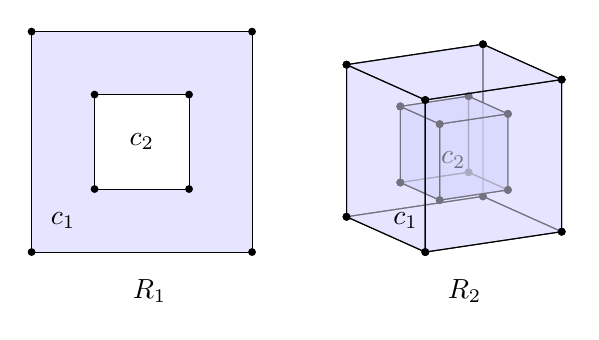
\begin{tikzpicture}
    \begin{scope}[region style,x=0.4cm, y=0.4cm]
        \filldraw[rnode] 
            (0, 0) node{} -- (7, 0) node{} -- (7, 7) node{} -- (0, 7) node{} -- cycle
            (2, 2) node{} -- (2, 5) node{} -- (5, 5) node{} -- (5, 2) node {} -- cycle;
        \path (1, 1) node{$c_1$};
        \path (3.5, 3.5) node{$c_2$};
    \end{scope}
    \begin{scope}[3d view, region style, xshift=5cm]
        \def\surface[#1,#2]{
            \fill[opacity=0.5] (#1, #1, 0) node{} -- (#2, #1, 0) node{} -- (#2, #2, 0) node{} -- (#1, #2, 0) node{} --cycle;
            \draw[rnode] (#1, #1, 0) node{} -- (#2, #1, 0) node{} -- (#2, #2, 0) node{} -- (#1, #2, 0) node{} -- cycle;
        }
        \def\threesides[#1,#2]#3{
            \begin{scope}[canvas is zy plane at x=#1, fill=#2]
                #3
            \end{scope}
            \begin{scope}[canvas is zx plane at y=#1, fill=#2]
                #3
            \end{scope}
            \begin{scope}[canvas is xy plane at z={2 - #1}, fill=#2]
                #3
            \end{scope}
        }
        \threesides[2,blue!20]{\surface[0,2]};
        \threesides[1.5,blue!40]{\surface[0.5,1.5]};
        \threesides[0.5,blue!10]{\surface[0.5,1.5]};
        \path (0.7,0.5,1) node {$c_2$};
        \threesides[0,blue!10]{\surface[0,2]};
        \path (0,0.5,0.3) node {$c_1$};
    \end{scope}
    \path (1.5, -0.5) node{$R_1$};
    \path (5.5, -0.5) node{$R_2$};
\end{tikzpicture}
\end{center}
\caption{A drawing of a 2 dimensional region $R_1$ and a 3 dimensional region $R_2$, both with two cells, $c_1$ and $c_2$.}
\end{figure}


A cell $c$ consists of a set of faces $F(c)$.
A face $f$ is a region $R_f$ in a subspace of $\mathcal{S}$. 
We call the faces of the cells in $R_f$ \emph{edges}.
A cell has two constraints:
The first is that each edge $e$ of each face $f_a$ is shared with exactly one other face $f_b$.
The second is that for each face $f_a$ there exists no other face $f_b$ such that the subspaces of $f_a$ and $f_b$ has an intersection that \emph{crosses} both $f_a$ and $f_b$.
We say that an intersection $I$ crosses a region $R$ if it intersects with any edges in $R$.
Alternativly we also say that an intersection $I$ crosses a region $R$

Given a cell $c$ of a region $R$ in a space $\mathcal{S}$ and an intersection of $\mathcal{S}$, $I$, we can compute the intersection of $R$ and $I$, known as $R_I$.

A face $f$ is a region $R_f$ in an subspace $\mathcal{B}$ of $\mathcal{S}$.
The edges of a face $f$ is the 

A cell $c$ also segments a space in the same way as its coresponding region, but it has some additional constraints. A cell consists of a set of  with the requirment that for each edge of a face

\section{Topological regions}

\section{Geometric robustness}
% See: https://people.eecs.berkeley.edu/~jrs/meshpapers/robnotes.pdf

\section{Planar geometry}

\subsection{Representation of lines and planes}
\subsection{Intersections of lines and planes}

\section{NURBS geometry}

\end{document}
